\documentclass{article}

\usepackage[utf8]{inputenc}
\usepackage{graphicx}
\usepackage[french]{babel}
\usepackage{hyperref}
\usepackage[top=2cm, bottom=2cm, left=2cm, right=2cm]{geometry}

\title{Rapport de projet web}
\author{Alexandre Garand, Lucas Bourel, Corentin Guillerme, Maxime Song}

\begin{document}
\maketitle
\setcounter{tocdepth}{2}
\tableofcontents
\newpage

\section{Présentation du projet}
    Notre projet est un site de réservation de trajets entre plusieurs villes (type uber). Mais au lieu de réserver un trajet en voiture, les utilisateurs réservent des trajets sur des créatures fantastiques (licornes, dragons, phénix ...).
    \\
    
    Les utilisateurs peuvent donc s'inscrire soit pour réserver un trajet soit pour proposer un trajet en tant que monture.
    \\
    
    Bien évidemment les trajets proposés n'existent pas dans la réalité.
    \\
    
    Par la suite les utilisateurs qui cherchent un trajet seront appelés des clients et ceux qui proposent de faire des trajets seront appelés des vendeurs, transporteurs, créatures ou montures.

\section{L'architecture}
	Nous avons choisit d'utiliser une structure modèle-vue-contrôleur.\\ \\
	Nous avons un fichier index.php qui est un routeur dirigeant vers toutes les pages du sites et est le seuls point d’accès de ces pages.\\ \\
	Ensuite nous avons un fichier template.php qui donne la structure de toutes les pages du sites contenant notamment l'en tète et le pied de la page.\\ \\
	Ensuite pour chaque page nous avons un fichier de vue contenant le contenue spécifique de la page.\\ \\
	Pour chaque page non-statique nous avons un fichier contrôleur qui décide quoi afficher pour ces pages en fonction du contexte.\\ \\
	Pour chaque table de la base de donnée nous avons un fichier avec une classe représentant la table avec les mêmes attributs et des accesseur et mutateurs pour modifier la classe et un fichier manager manipulant la base de donnée et la classe php pour permettre d'accéder et traiter les données.\\ \\
	Le principe du site web est donc d'avoir index.php qui appelle le contrôleur de la page web à afficher, le contrôleur peut utiliser les classes du modèle pour manipuler la base de donnée puis il envoie la vue de la page à afficher à template.php qui affiche la page.
\section{Le modèle}
	\subsection{Les bases de données}
		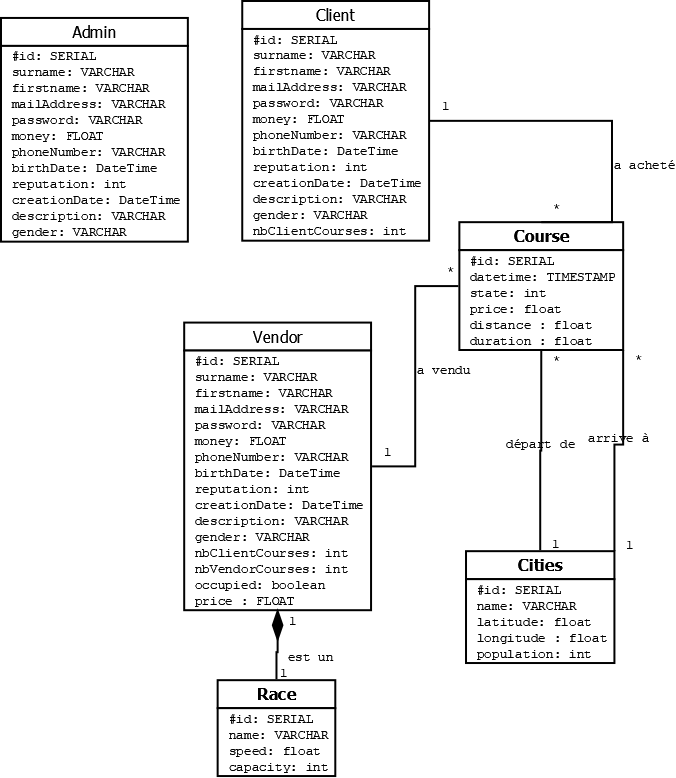
\includegraphics[scale=0.3]{diagrammeTotal.png} \\
		\subsubsection{Admin/Client/Vendor}
			Ces trois tables représentent les utilisateurs selon leur rôle et contient toutes les informations afin de permettre l'utilisation du sites ainsi que des informations classiques sur les utilisateurs. Il est important de noter que le vendeur est peut aussi utiliser le site en tant que client.
		\subsubsection{Race}
			Cette table contient le nom et les caractéristique de la race afin de savoir comment les clients serons servis par la race en question.
		\subsubsection{Course}
			Celle-ci contient les informations sur les transports effectués afin de permettre aux utilisateurs d'accédés à l'historique de leurs transactions.
		\subsubsection{Cities}
			Celle-ci contient les informations sur les villes: les coordonnées gps pour pouvoir les placés et la population pour pouvoir les trier dans la liste des propositions pour l’auto-complétion.
	\subsection{Le programme}
		\subsubsection{Principe général}
			Pour chacune des tables de la base de donnée afin de pouvoir les manipuler efficacement en php chaque table est représenter par une classe possédant les mêmes attributs que la bases de donnée, un accesseur pour chaque attribut et un mutateur pour chaque sauf ceux qui ne doivent pas être modifier tels que l'id ou la date de création d'un compte.
		\subsubsection{Cas particulier de User}
			Une classe de plus à été ajouter au modèle: la classe User.\\ Celle-ci est la classe mère de Admin Client et Vendor permettant de ne pas avoir à réécrire la même chose trois fois pour chaque attribut en commun pour les trois.
		\subsubsection{Les managers}
			Les managers permettent de lire la base de donnée et de convertir une ligne de la table en une instance de la classe correspondant et vis-versa : elle permet d'ajouter, de détruire, de modifier ou d'accéder à une ligne de la base de donnée ou d'accéder à toutes les lignes. Il y à aussi des opérations spécifiques à certaines tables comme dans Cities qui à une fonction spécifique pour l'auto-complétion allant chercher les villes commençant par une chaîne de caractère.
	\subsection{Problèmes rencontrés et solutions}
		\subsubsection{Les injections SQL}
			Un problème que nous avons eu est la possibilité d'effectué des injections SQL en effet avec la fonction query l'utilisateur pouvait utiliser la chaîne de caractère qu'il voulait pour faire faire ce qu'il voulait à la base de donnée.\\ Pour palier à ce problème nous avons utiliser la fonction prepare qui empêche ce genre d'acte malveillant.
		\subsubsection{Les injections SQL}
			Le deuxième problème rencontrer est l'héritage de User qui n'a pas pus être fais au niveau de la base de donnée ce qui à été pallié en écrivant trois base de donnée distincte avec des données similaires. Cette solution peu efficace à causer une duplication du code importante et un héritage peu utile au niveau des managers.
			
\section{Réservation de trajet}
    \subsection{Partie client}
        Pour réserver un trajet les utilisateurs ont à disposition un formulaire dans lequel ils entrent la ville de départ et la ville d'arrivée.
        
        Ils arrivent ensuite sur une page avec la liste des créatures pouvant effectuer ce trajet avec des informations comme le prix et le temps de trajet.
        
        En choisissant un trajet ils arrivent sur une page affichant des informations plus complètes sur le trajet et un lien vers le profil public du vendeur.
        
        Sur cette page ils peuvent réserver le trajet puis sont inviter à entrer un numéro de carte bancaire pour confirmer le paiement.
        \\
        
        Le client est alors informé par mail que son trajet à bien été réservé et obtient un lien pour accéder à des informations sur ce dernier.
        
        Dès que le vendeur a accepté (ou refusé) le trajet le client en est informé par un mail.
        \\
        
        Le client peut annuler un trajet à tout moment excepté si ce dernier est déjà terminé.
    
    \subsection{Partie Vendeur}
        Lorsqu'un client a fait une demande de réservation, le vendeur correspondant est alerté par mail qui contient un lien vers ce trajet et de là il peut soit accepter soit refuser. Le client recevra alors un mail l'informant de sa décision.
        \\
        
        Par la suite le vendeur aura toujours la possibilité d'annuler le trajet avant que celui-ci ne se termine.
            
            
    \subsection{Problèmes rencontrés et solutions}
        \subsubsection{Envois de mails}
            Afin d'informer les utilisateurs sur les états des réservations la façon la plus simple étant donné qu'ils peuvent ne pas être connecté au site est de leur envoyer des mails.
            \\
            
            Pour cela nous avons du installer PHPMailer afin de faciliter l'envoi de mails.
            Dans l'objectif dene pas mettre les identifiants et mots de passe du compte mail utilisé pour les envois dans le code source PHP nous avons utilisé XOAUTH2 pour se connecter.
            \\
            
            Le compte mail utilisé est un compte GMail car il nous permet d'avoir accès à une quantité illimitée d'alias ce qui est beaucoup plus pratique pour les phases de test.
        
        \subsubsection{Affichage du trajet sur une carte}
            Pour afficher une carte avec le trajet effectué nous avons utilisé l'API Leaflet car elle est très légère, gratuite et opensource.
            \\
            
            Les cartes proviennent d'OpenStreetMap et le chemin parcourru a été obtenu grâce à openrouteservice. Cependant ce service nécessitant une clé pour être utilisé nous avons du mettre la requete au niveau du PHP pour éviter que les utilisateurs ne voient la clé utilisée.
            La requète se fait à l'aide d'Ajax car cela permet de réduire le temps de réponse du serveur pour l'envoi de la page.
        
        \subsubsection{Formulaire de choix des villes}
            Afin d'avoir des villes pour les départs et les arrivées nous avons récupéré une liste de ville qui provient de geonames.
            
            Pour faciliter le choix de la ville nous avons du en supprimer certaines de la base de bonnées pour éviter qu'il n'y ait plusieurs villes ayant le même nom (nous avons gardé celle ayant le plus d'habitants)
            \\
            
            Pour que l'utilisateur puisse plus facilement choisir une ville nous avons ajouté un script d'autocomplétion qui affiche à l'aide d'Ajax une liste déroulante contenant des noms de villes commençant par ce que l'utilisateur a entré.
            
            Cependant comme le serveur n'accepte qu cinq connexions à la fois nous avons qu ajouter un timeout avant de faire la requête pour vérifier si la valeur du champ a changé et ainsi limiter le nombre de requêtes pour ne pas faire planter le serveur.
        
        \subsubsection{Stockage des trajets}
            Il est impossible de stocker tous les trajets qui peuvent être effectués car il est de l'ordre du nombre de vendeurs sur des villes différentes multiplié pas le nombre de villes (on arrive très rapidement au dessus du million). 
            \\
            
            Pour les recherches de trajets on regarde donc quels vendeurs sont disponibles à la ville de départ et on crée un trajet pour chacun d'entre eux mais sans le rajouter à la base de donnée. Ils ne sont entrés que lorsque le client arrive sur la page de paiement, pour éviter qu'ils ne soient modifiés pendant le paiement.
        
        \subsubsection{Calcul de distance entre les villes}
            Comme l'API de recherche de chemin entre deux villes est limitée à des chemins inférieurs à 6 000 km et qui ne traversent pas les océans il faut utiliser une autre méthode pour calculer les distances entre deux villes.
            
            C'est pour cela que les distances sont calculées à l'aide des coordonnées GPS.
            
    \section{L'espace membre}
Il a fallu gérer les deux types d'utilisateurs du site web, les transporteurs et les clients. Profitant de la configuration MVC, et puisque tout demande de passage passait par le routeur index.php, on a mis en place un petit fichier de configuration config.php pour y définir certaines variables globales utiles dans tout le reste du code. 
\\
\\
Tout d'abord, lors de la connexion de l'utilisateur, on stock certaines informations dans les variables de sessions. Mais, on s'était vite rendu compte qu'en y stockant l'objet PHP représentant la donnée user, on perdait la spécificité de la classe fille utilisé. 
\\ 
On a donc choisi plutôt en solution de seulement stocker l'id ainsi que le type d'utilisateur. Avec seulement ce couple d'information, on pouvait savoir où chercher et dans quelle tables pour retrouver l'utilisateur actuelle. Ce couple d'informations est donc stocké dans les variables de sessions. De plus, on charge dans le fichier de configuration config.php directement en tant que variable globale cette fois, la variable objet utilisateur correspondant à l'utilisateur actuelle. 

\subsection{Différents utilisateurs} 
On distingue les trois types d'utilisateur, correspondant au trois tables du modèle. Les transporteurs (ou vendeurs), les clients, et les administrateurs.
Se sont posées les problématiques des multi-comptes ainsi que celui de l'utilisateur possédant différentes casquettes. 
\\
Il a été choisi, dans le but de simplifier le modèle de donnée, de limiter un compte utilisateur par adresse mail, peu importe la nature de ce compte. 
Autrement dit, une adresse mail employé dans un compte client ne peut être utilisé pour un compte vendeurs. 
\\
On s'est toutefois laissé la possibilité de considérer les vendeurs comme des utilisateurs clients améliorées. Enfin, concernant les admins, leur particularité est surtout de leur permettre d'avoir accès à une partie du site leur procurant certaines fonctionnalité supplémentaire avec un accès sur le reste des bases de données.

\subsubsection{Inscription}
Seul l'inscription pour les deux premiers types d'utilisateurs sont disponible de manière public. Puisque les données à y inscrire sont légèrement différents, deux contrôleurs différents ont été fait, l'une pour l'inscription client, l'autre pour l'inscription vendeur. 
\subsubsection{vérification des données}
\\
La vérification des données entrées par l'utilisateur, notamment pour le format de l'adresse mail, de la date de naissance et du numéro de téléphone ont été effectué côté serveur ( à l'aide d'expression régulières).  
De plus, on a rajouté un script javascript permettant de manière plus dynamique de vérifier ces entrées pendant la saisie des données. On a ainsi placé dans la vue, un message de rappel sur le format des entrées, pour les champs qui le nécessitait. Un script javascript ne rendait visible que les indications pour les champs venant d'être modifié et ne remplissant pas ses contraintes. 
\\
Bien sûr, la vérification javascript s'effectue côté client et n'est absolument pas une méthode sûr pour s'assurer des données. 
\subsubsection{Choix de la race pour le transporteur} 
Un deuxième problème s'est posé quand au choix de la race. Concernant le contrôleur associé au vendeur, il fallait pouvoir disposer des races ainsi que des informations les concernant. Soit, donc du côté php, un appel au modèle pour pouvoir disposer de la liste des races disponibles.
Mais c'est encore une fois un script javascript qui a été choisi pour afficher seulement les informations relatives à la race sélectionné pendant la saisie de l'utilisateur. 
\\
Par contre, cette fois-ci, si le script n'arrive pas à s'exécuter, on considère comme non nécessaire ces informations. L'utilisateur pourra toujours choisir sa race, même si l'affichage dynamique ne lui permettra pas de voir ses caractéristiques. 

\subsection{La connexion}
Puisqu'il a été choisi d'unifier l'unicité de l'adresse mail pour les trois types d'utilisateurs, une seul page de connexion pour ces trois utilisateurs différents suffit. 
C'est une fonction commune aux trois manager, permettant de vérifier la présence d'un couple d'identifiant/motdepasse dans une des trois base de données. 
\\
D'ailleurs, concernant le stockage de ces mots de passe dans la base de donnée, c'est posé également la question de sécurité. On a du bien sûr, hasher les mots de passe de nos utilisateurs, c'est à dire les passer à travers un algorithme de cryptage tel qu'il est facile de vérifier l'égalité avec un autre mot de passe en lui faisant passer le même processus mais beaucoup plus dur à partir des simples données de la base de donnée duquel on a accès retrouverez le mot de passe. 
\\ Concernant le hashage utilisé, on a décidé de se fixer sur la méthode standard défini par les normes de PHP, soit verify_password() et hash_password(), fonction qui ont l'avantage d'évoluer régulièrement et de ne pas se limiter qu'à un seul type de hashage. 
\\
\subsection{Le profil} 
L'ensemble des utilisateurs partageant la même base concernant leur représentation. Tous possèdent une adresse mail, un numéro de téléphone, une date de naissance, .... Ainsi, concernant la gestion de leur profil, similaire donc, un seul contrôleur a été fixé, rajoutant des champs au formulaire si besoin. 
\\  C'est donc à cette partie commune à tous les utilisateurs que la connexion commune ramène. 
\\
Le choix a été fait d'avoir accès à un formulaire dont la modification a été désactivé. Grâce à un bouton, on peut ouvrir à la modification le formulaire. \\
Trois choix s'offrent ensuite à l'utilisateur. Soit valider les modifications qu'il a fait, soit revenir à l'état précedent mais rester en état de modification des champs, soit annuler ses changements et revenir à l'état du formulaire figé à l'image des données utilisateurs actuelles. \\ \\
Toujours concernant le vendeur, s'est posé la même question concernant le choix de la race, et le script javascript d'information associé  a été renouvelé dans cette partie. 

\subsection{Paramètres du compte}
On était proposé dans cette partie, pour tous les utilisateurs, la possibilité de changer de mot de passe ou alors de tout simplement détruire leur compte. 
Les liens vers lequel cet utilisateurs s'était attaché ramèneront alors vers une page pour les utilisateurs désormais inexistants. Il devient Inconnu lors des affichages. 

\subsection{Mes Trajets}
Deux partie se distingue alors selon les utilisateurs, bien que la vue pourtant reste identique. 
Du côté des utilisateurs clients, on affiche un tableau représentant l'ensemble des trajets qu'ils ont effectué en tant que client. 
\\
Du côté des vendeurs, ce sera l'ensemble des trajtes effecuté en tant que vendeur qui sera affiché. 
\\ 
Soit, seulement finalement l'appel à la base de donnée change réellement quelque chose entre ces deux types. 
Cette espace n'est pas particulièrement destinée à l'admin qui a le droit lui de consulter l'ensemble des trajets. 

\\subsection{Déconnexion}
Il s'agit d'une page de déconnexion commune à tous. Elle s'occupe seulement de se vider des variables de sessions, ains que des variables globales. 

\subsection{L'espace Admin}

L'espace admin laisse la possibilité d'accéder à la liste des clients enregistré sur le site. On peut modifier ce qui concerne la partie profil de cette utilisateurs. 
On peut également détruire ce compte, mais il s'agit d'une opération dangereuse. En effet, tel qu'implementé actuellement, il n'y a pas vérification et suppression de la présence de cet utilisateur dans les autres bases de données.
\\
La même possibilité est laissé pour la liste des vendeurs. Toutefois, on ne peut pas modifier les caractéristiques de leur profil spécifique à leur aspect vendeur. 
\\
L'admin a également la possibilité d'accéder à l'ensemble des trajets dans la base de données. 
Enfin, il est le seul à pouvoir rajouter une nouvelle race dans la base de donnée, ainsi qu'un nouvel admin.

\subsection{configuration du template}
Pour pouvoir accéder à l'espace membres et les différentes pages que l'on vient de proposer, il faut que cela soit accessible.  
En s'aidant des variables de sessions et de celles défini dans config.php, il est facilement possible dans la page template d'y inclure un menu supplémentaire pour accéder à ses pages, selon le degré de connexion et le type de connexion , permettant à l'utilisateur connecté de disposer de son menu correspondant. 
Le menu vendeur et client reste le même, ( car c'est le contrôleur de la modification du profil, et de la liste des trajets qui s'occupe de la distinction ) 

\section{La vue}

\section{Possibles amélioration}
Certaines tables dans la base de données et ainsi que des manager dans le modèle existe mais ne sont pas utilisé. 
Elle corresponde à des fonctionnalitées envisagés au début du projet mais qui ont été abandonné par la suite. 
Ainsi, on était envisagé la possibilité pour les utilisateurs de commenter les vendeurs et d'établir ainsi un score de réputation. 
\\
Dans la partie admin, la possibilité de modifier les aspects vendeur ( race, position, occupé) des transporteurs. 
Enfin, la possibilité de demander l'ajout d'une race par un utilisateur ( devant ensuite être validé par l'un des admins)

\section{La répartition des rôles}
\begin{description}
 \item[Alexandre Garand :]. Le modèle pour les tables Admin, Client, Vendor, Cities, Race 
 \\
 
 
 \item[Lucas Bourel :] . Toute la partie concernant l'espèce membres (inscription, connexion, déconnexion, modification du profil et des paramètres) ainsi que l'espace admin. Au niveau du contrôleur et de la vue. 
 \\
 
 \item[Corentin Guillerme :] toute la partie réservation de trajets côté controller et vue (recherche de trajets, réservation, envois de mails...)
 \\
 
 \item[Maxime Song :].
 \\
\end{description}

\section{Informations complémentaires}
    \subsection{Modules installés}
        Afin de pouvoir envoyer des mails nous avons du installer PHPMailer et league/oauth2-google. Pour cela nous avons inclus ces modules dans le fichier composer.json pour qu'ils soient installés automatiquement lors d'un $make install$
        
    \subsection{réécriture des URLs}
        Notre site utilise le fichier index.php comme routeur donc toutes les demandes de pages passent par ce fichier avec une adresse du type adresseDuSite/index.php?action=truc
        
        Afin d'avoir des URLs plus jolies nous avons modifié le fichier de configuration du serveur (.docker/nginx-php/config/site.config) pour ajouter des réécritures d'URL.
        
        Toutes les URLs de la forme adresseDuSite/truc sont donc réécrites au niveau du serveur en adresseDuSite/index.php?action=truc
        \\
        
        Cela permet d'avoir de belles URLs au niveau de l'utilisateur.
        
    \subsection{bots}
        Le nombre de villes présentes dans la base de données est de l'ordre de 160 000. Donc pour éviter de ne pas trouver de trajet dans la grande majorité des cas il faudrait remplir la base de données avec un nombre de vendeurs du même ordre de grandeur de le nombre de villes. Pour éviter cela des vendeurs sont automatiquement ajoutés à la base de données à chaque recherche de trajet.
        
        Ce comportement est désactivable en passant la variable $\$modeDemo$ à false dans le fichier config.php.
        
    \subsection{identifiants}
        compte admin : admin@uber-licorne.com / 
        
        comptes bots : testprojetlicorne+bot_<id_aléatoire>@gmail.com / imabot
        
        compte gmail : testprojetlicorne@gmail.com / 159asxcv
        
\end{document}
